
\subsection{GPU acceleration reduces design runtimes}

The vast majority of \osprey runtime in designs with continuous flexibility is spent minimizing protein conformations and conformation fragments. Although the runtimes of sufficiently large designs can be dominated by the exponential-time worst case performance of the A* search phase, if the A* phase can be completed within an acceptable time limit, the merely polynomial-time conformation minimization phase still often dominates the total run time because conformation minimization is a computationally-expensive and time-consuming function {\it per-operation} compared to scoring nodes in the A* tree. In other words, even though we need to do an exponential amount of work to select leaf nodes in the A* tree corresponding to the low-energy conformations of the design, examining A* nodes is relatively inexpensive. Minimizing the conformations associated those same A* leaf nodes to calculate their true forcefield energies is much more expensive, and can take far more time overall. Therefore, methods that increase protein conformation minimization speeds can have a dramatic impact on \osprey runtimes in cases where the A* search time is acceptable.

Much work has been done in the past to optimize \osprey for execution on CPUs, particularly highly multi-core CPUs and even networked clusters of CPU-powered servers \jeff{add some citations here?}. However, modern GPU hardware enables high-performance computation at a fraction of the cost of large CPU clusters, mainly due to the huge video game industry that propels innovation in hardware design and drives down costs. \osprey3 includes GPU programs (called {\it kernels}) built using the CUDA framework that implements the forcefield calculations and local minimization algorithms used in protein redesign. We present performance results of these GPU kernels on various hardware platforms in Figure~\ref{fig:gpu}. Overall, on desktop-class machines, GPU hardware improves minimizations speeds over multi-core CPUs by roughly 12-fold for sufficiently large molecules. On server-class machines, a single GPU is merely about 2.6-fold faster than dual CPUs. These large machines can house more GPUs than CPUs though, so a fully-provisioned server with 4 or even 8 GPUs would likely greatly outperform 2 or even 4 CPUs. \jeff{It's super hard to get good multi-GPU benchmark data on the shared CS machines. Hopefully a speculative statement about multi-GPU performance is good enough here?}

Modern GPU architectures offer thousands of parallel hardware units for calculations, compared to the tens of parallel hardware units in modern CPU architectures. The performance results of the current incarnation of \osprey's GPU kernels indicate that current minimization speeds on GPUs have only begun to scratch the surface of what is possible, particularly for molecules with a small number of atom pairs. It is incredibly likely that future versions of these GPU kernels will offer significantly higher performance on the same hardware -- perhaps allowing minimization speeds many times faster than today's GPU kernels.

\begin{figure}\label{fig:gpu}
\center
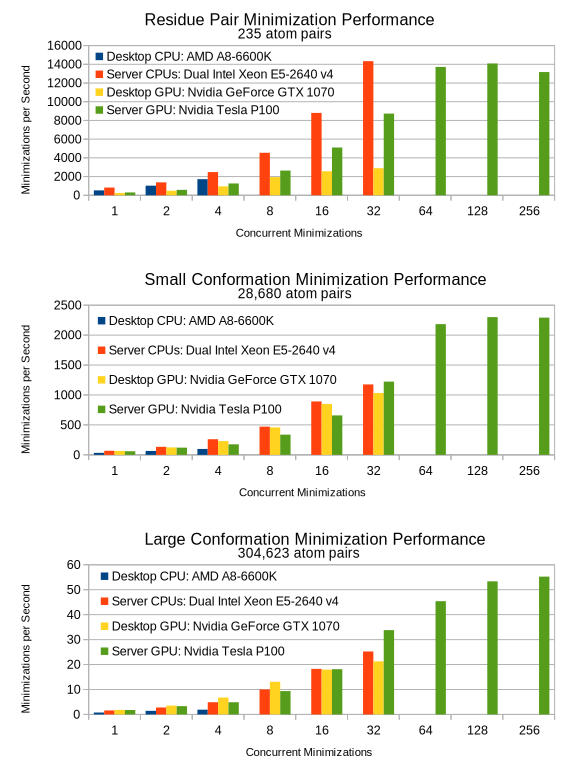
\includegraphics[width=4in]{figures/gpu.pdf}

\jeff{This figure turned out kind of big. Is there room for it? Should we cut some results? Or present them differently?}
\caption{Benchmarks for protein conformation minimization in \osprey3 for various hardware platforms and for molecules of varying size. From smallest to largest: {\bf (top)} a single residue pair used in energy matrix computations, {\bf (middle)} a full protein conformation with a single flexible residue, {\bf (bottom)} a full protein conformation with 20 flexible residues. For CPU hardware, concurrent minimizations correspond to CPU threads. For GPU hardware, concurrent minimizations correspond to {\it streams} defined by the CUDA framework. Faster minimization speeds correspond with faster \osprey runtimes.}
\end{figure}
